\chapter{JPEG2000}
\label{cha:JPEG2000}

\section{\glsentryshort{ISO} international standard}
\begin{itemize}
\item Developed by the \gls{JPEG} (ISO/IEC 15444\href{https://www.itu.int}{ITU}),
  the JPEG2000 standard \cite{taubman2002jpeg2000,wikipedia_J2K} in 2000, as a successor of
  \gls{JPEG}.
\item Mainly used in medical imaging and digital cinema.
\end{itemize}

\section{Lossless and lossy compression}
\begin{itemize}
\item Two different compression modes:
  \begin{enumerate}
  \item \textbf{Reversible}: Allows a perfect reconstruction of the raster image (like \gls{PNG}).
  \item \textbf{Irreversible}: Unable to recover all the visual
    information, but offers a better rate/distortion performance than
    the reversible mode for the same bit-rate.
  \end{enumerate}
\end{itemize}

\section{16-bit per channel and several color spaces support}
\begin{itemize}
\item \popup{16 bits/pixel offers enough quality for specialized
  applications such as medicine, astronomy, etc}{It is quite difficult
  to increase the SNR above of 16 bits because basically we register
  noise when the amplitude of signal is small.}.
\item Apart from gray-scale and \gls{RGB}, JPEG2000 supports
  \gls{YCbCr}, \gls{sRGB} \cite{sRGB_wikipedia}, \gls{CIELAB}
  \cite{CIELAB_wikipedia}, and \popup{custom}{It is posible to define
    a color transform.} \cite{houchin2001specification} color spaces.
\end{itemize}

\section{Superior compression efficiency than \gls{JPEG}}
\begin{itemize}
\item Better quality at the same bitrate compared to JPEG \cite{vruiz_J2K}.
\end{itemize}

\begin{figure}[H]
  \vspace{-2ex}
  \centering
  \begin{tabular}{cc}
    \multicolumn{2}{c}{Lena at 0.1 bits/pixel} \\
    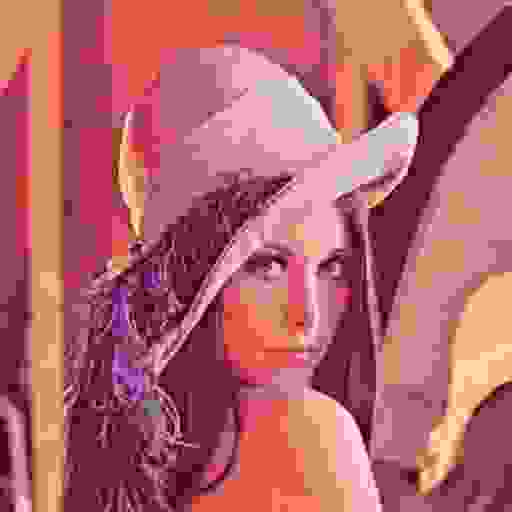
\includegraphics[width=5cm]{lena_01} & 
\includegraphics[width=5cm]{lena_01_jp2} \\
    JPEG & JPEG2000
  \end{tabular}
  \caption{\gls{JPEG} VS JPEG2000.}
  \label{fig:J2K_JPEG}
\end{figure}

\section{Baseline algorithm}
\begin{enumerate}
\item Convert from the \gls{RGB} color space to the \gls{YCbCr} color
  space. Only if the input image is in color and not in \gls{YCbCr}.
\item Transform each \gls{YCbCr} component using the 2D-\gls{DWT}.
\item If we are using the irreversible mode, quantize the \gls{DWT}
  coefficients. /* Lossy step */
\item Entropy encode the quantized coefficients with \gls{EBCOT}.
\end{enumerate}

\section{Structure of an image in the DWT domain}
\begin{itemize}
\item The \gls{DWT} represents signals as a multiresolution structure
  \cite{vruiz_J2K}.
\end{itemize}

\begin{figure}[H]
  \vspace{-2ex}
  \centering
  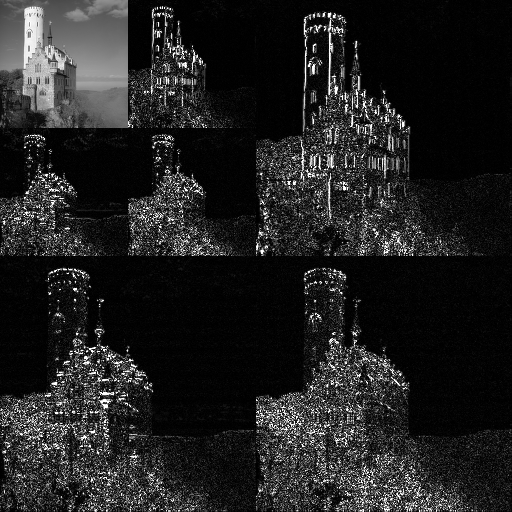
\includegraphics[width=6cm]{2-level_wavelet_transform-lichtenstein}
  \caption{A 2-levels \gls{DWT} decomposition of an image.}
  \label{fig:J2K_DWT}
\end{figure}

\section{Spatial scalability}
\begin{itemize}
\item When the image is rendered by resolution levels.
\end{itemize}

\begin{figure}[H]
  \vspace{-2ex}
  \centering
  \resizebox{11cm}{!}{
    \begin{tabular}{ccc}
      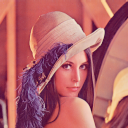
\includegraphics{lena_128x128_rgb} & 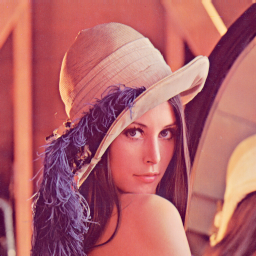
\includegraphics{lena_256x256_rgb} & 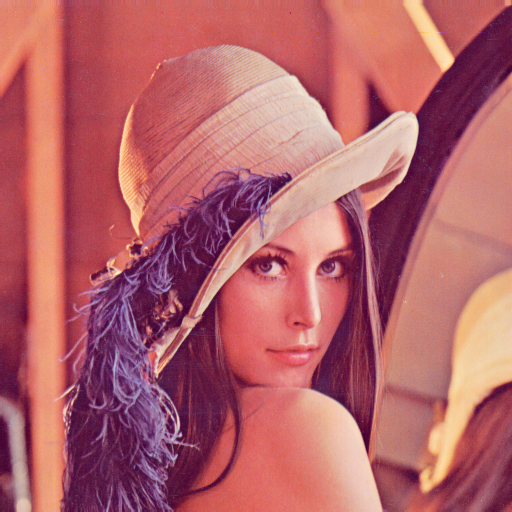
\includegraphics{lena_512x512_rgb}
    \end{tabular}
  }
  \caption{Spatial scalability provided by JPEG2000.}
  \label{fig:J2K_spatial}
\end{figure}

\section{Quality scalability}
\begin{itemize}
\item When the image is rendered by \popup{coefficient amplitude}{DWT
    coefficients are actually decoded based on their contribution to
    the rate/distortion (R/D) curve. An R/D curve relates (X-axis) the
    amount of decompressed data versus (Y-axis) the achieved
    distortion. Depending on the distortion metric used, the curve may
    decrease with increasing number of decompressed bits (e.g., when
    measuring MSE) or increase with increasing number of decompressed
    bits (e.g., when measuring SNR).} \cite{vruiz_J2K}.
\end{itemize}

\begin{figure}[H]
  \vspace{-2ex}
  \centering
  \resizebox{11cm}{!}{
    \begin{tabular}{ccc}
    
\includegraphics[width=4.0cm]{lena_01_jp2} & 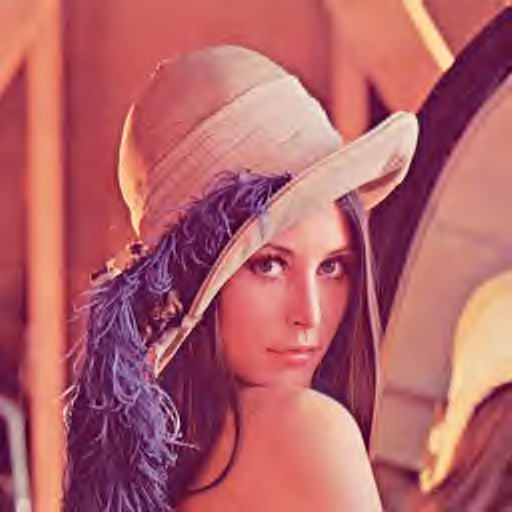
\includegraphics[width=4.0cm]{lena_02_jp2} & 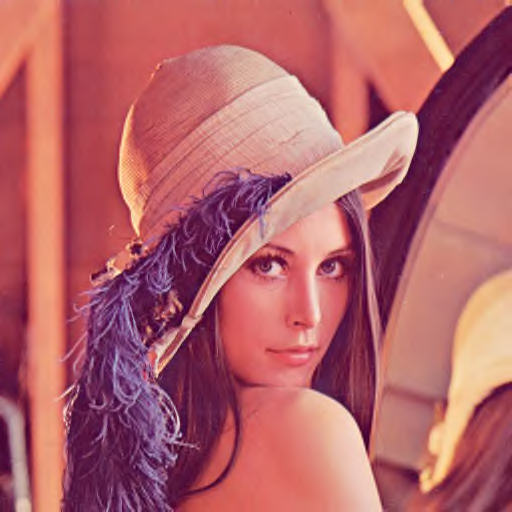
\includegraphics[width=4.0cm]{lena_05_jp2} \\
    0.1 bits/pixel & 0.2 bits/pixel & 0.5 bits/pixel
    \end{tabular}
  }
  \caption{Quality scalability provided by JPEG2000.}
  \label{fig:J2K_quality}
\end{figure}

\section{\acrshort{ROI} scalability}
\begin{itemize}
\item It is possible to dedicate more bit-rate to a \gls{ROI}, that
  can be defined interactively \cite{vruiz_J2K}.
\end{itemize}

\begin{figure}[H]
  \vspace{-2ex}
  \centering
  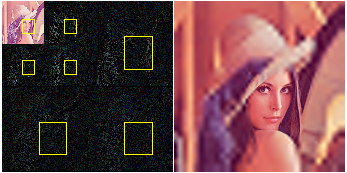
\includegraphics[width=11cm]{ROI}
  \caption{\gls{ROI} scalability provided by JPEG2000.}
  \label{fig:J2K_ROI}
\end{figure}
  
\section{Error resilience}
\begin{itemize}
\item An error in JPEG 2000 tends to affect only localized image areas
  rather than corrupting the entire picture, due to the entropy coding
  of data in relatively small independent blocks
  \cite{wikipedia_J2K,brahimi2021efficient}.
\end{itemize}

\begin{figure}[H]
  \vspace{-2ex}
  \centering
  \href{https://flylib.com/books/en/2.537.1.37/1}{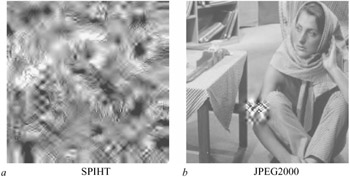
\includegraphics[width=11cm]{J2K_error_resilience}}
  \caption{Error ``correction'' provided by JPEG2000. A comparison
    with \gls{SPIHT} \cite{wikipedia_SPIHT}.}
  \label{fig:J2K_error}
\end{figure}

\section{3D support}
\begin{itemize}
\item Based on the 3D-DWT \cite{Bruylants_J2K_3D}.
\end{itemize}

\begin{figure}[H]
  \vspace{-2ex}
  \centering
  \href{https://spie.org/images/Graphics/Newsroom/Imported/0779/0779_fig1.jpg}{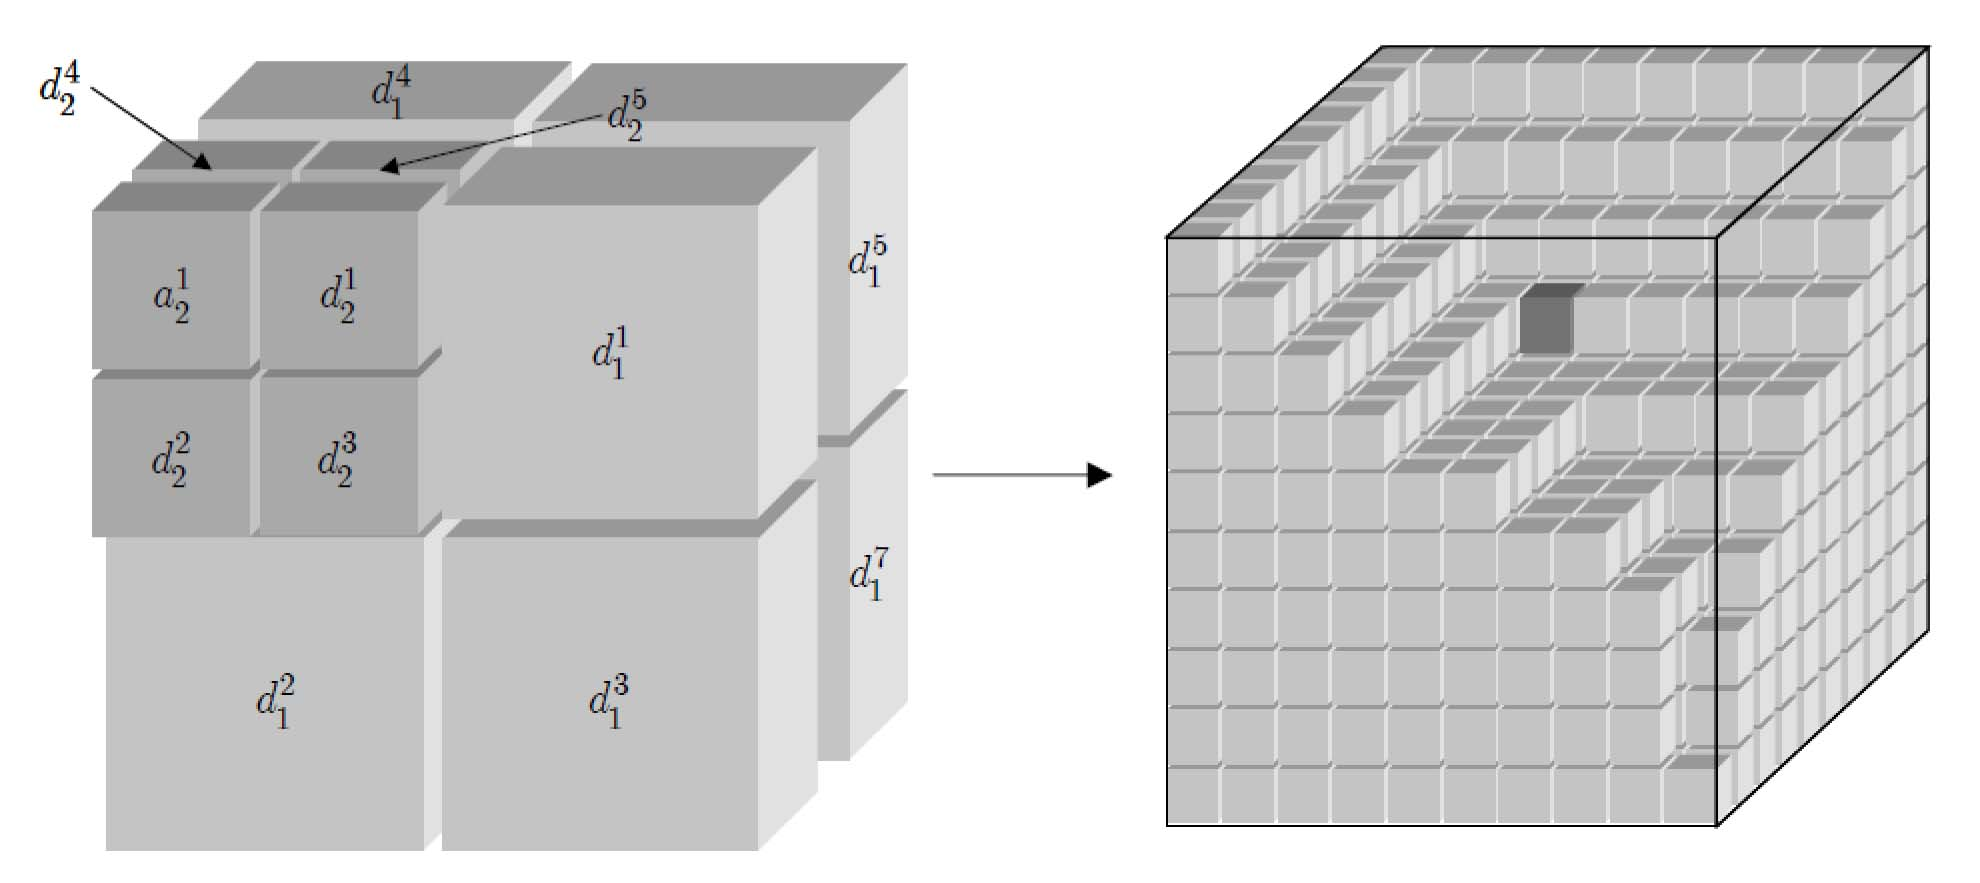
\includegraphics[width=11cm]{J2K_3D}}
  \caption{Processing of 3D images in JPEG2000.}
  \label{fig:J2K_3D}
\end{figure}

\section{Motion JPEG2000 (digital cinema)}
\begin{itemize}
\item The movies played in digital cinemas leverage the spatial
  scalability provided by JPEG2000 to distribute a single DCP file
  that can be played in different resolution-capability beamers
  \cite{wikipedia_DCP}.
\item Each piture of the movie is compressed independently
  \cite{DigitalCinema}.
\end{itemize}

\begin{figure}[H]
  \vspace{-2ex}
  \centering
  \href{https://vicente-gonzalez-ruiz.github.io/JPEG2000/}{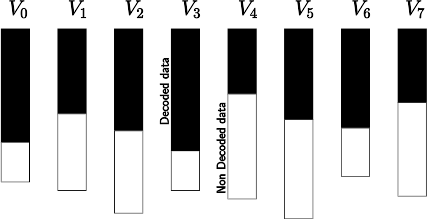
\includegraphics[width=8cm]{MJ2K}}
  \caption{In motion JPEG2000 the code-stream scalabiliy allow to
    adapt it to the context (for example, to the resolution of the
    display).}
  \label{fig:J2K_motion}
\end{figure}

\section{\glsentrylong{JPIP} ({\glsentryshort{JPIP})}}
\begin{itemize}
\item Based on the client/server model.
\item The client (the image viewer), \popup{interactively}{Usually
    controlled by a human.}, request to the server (that access to the
  JPEG2000 file \popup{locally}{Usually on a local disk.}) a sequence
  of \popup{\glspl{ROI}}{Actually, the term that the standard uses is
    ``WOI (Window Of Interest)''} \cite{ORTIZ04b}.
\item The server sends only those \popup{pieces of
    code-stream}{Data-bins} that are related with the current
  \gls{ROI} (which can be modified at any time). If the image is very
  big compared to the \gls{ROI}, this can save a lot of
  \popup{bandwidth}{In computer networks, bandwidth is a synonym of
    transmission capacity of the communication channel.}.
\end{itemize}

\begin{figure}[H]
  \vspace{-1ex}
  \centering
  \href{http://www.hpca.ual.es/~vruiz/papers/ORTIZ04c.pdf}{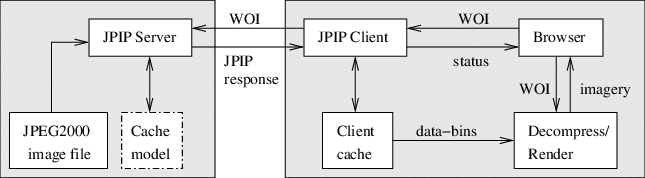
\includegraphics[width=10cm]{JPIP}}
  \caption{A desciption of \gls{JPIP}.}
  \label{fig:J2K_JPIP}
\end{figure}

\begin{figure}[H]
  \vspace{-1ex}
  \centering
  \href{https://ieeexplore.ieee.org/document/7214293}{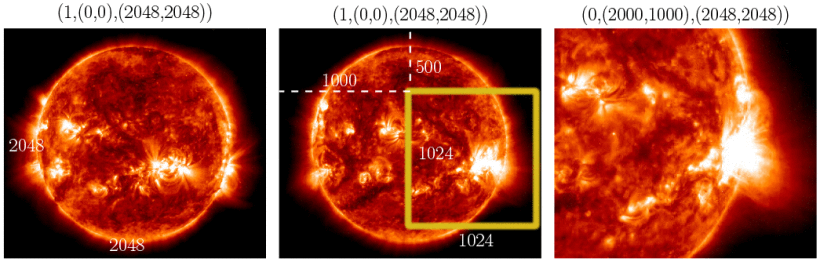
\includegraphics[width=\textwidth]{JPIP_example}}
  \caption{An example of an interaction with a JPEG2000 server using \gls{JPIP}.}
  \label{fig:J2K_motion}
\end{figure}

\section{Metadata}
\begin{itemize}
\item
  \href{https://github.com/vicente-gonzalez-ruiz/medical_imaging/blob/main/notebooks/JPEG2000_add_metadata.ipynb}{Here}
  there is an example that shows and modifies the metadata in a JPEG2000
  image.
\end{itemize}
